\begin{figure}[t]
\centering
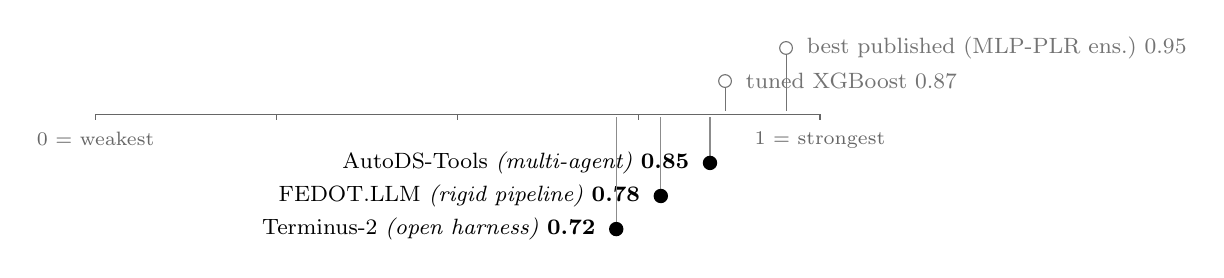
\begin{tikzpicture}[x=9.2cm,y=1cm]
\draw[black!60] (0,0) -- (1,0);
\draw[black!60] (0,0) -- (0,-0.07);
\draw[black!60] (0.25,0) -- (0.25,-0.07);
\draw[black!60] (0.5,0) -- (0.5,-0.07);
\draw[black!60] (0.75,0) -- (0.75,-0.07);
\draw[black!60] (1.0,0) -- (1.0,-0.07);
\node[font=\scriptsize,black!60,anchor=north] at (0,-0.10) {0 = weakest};
\node[font=\scriptsize,black!60,anchor=north] at (1,-0.10) {1 = strongest};
\draw[black!55] (0.8690,0.04) -- (0.8690,0.37);
\draw[black!55,fill=white] (0.8690,0.42) circle (2.3pt);
\node[font=\footnotesize,black!55,anchor=west,xshift=4pt] at (0.8690,0.42) {tuned XGBoost\ 0.87};
\draw[black!55] (0.9532,0.04) -- (0.9532,0.79);
\draw[black!55,fill=white] (0.9532,0.84) circle (2.3pt);
\node[font=\footnotesize,black!55,anchor=west,xshift=4pt] at (0.9532,0.84) {best published (MLP-PLR ens.)\ 0.95};
\draw[black!45] (0.8482,-0.04) -- (0.8482,-0.57);
\fill (0.8482,-0.62) circle (2.6pt);
\node[font=\footnotesize,anchor=east,xshift=-4pt] at (0.8482,-0.62) {AutoDS-Tools \emph{(multi-agent)}\ \textbf{0.85}};
\draw[black!45] (0.7803,-0.04) -- (0.7803,-0.99);
\fill (0.7803,-1.04) circle (2.6pt);
\node[font=\footnotesize,anchor=east,xshift=-4pt] at (0.7803,-1.04) {FEDOT.LLM \emph{(rigid pipeline)}\ \textbf{0.78}};
\draw[black!45] (0.7188,-0.04) -- (0.7188,-1.41);
\fill (0.7188,-1.46) circle (2.6pt);
\node[font=\footnotesize,anchor=east,xshift=-4pt] at (0.7188,-1.46) {Terminus-2 \emph{(open harness)}\ \textbf{0.72}};
\end{tikzpicture}
\caption{The three architectures (below the line) against the two marks that matter (above it), on the normalised scale where $0$ is the weakest and $1$ the strongest of the eighteen published baselines on each task. One backbone throughout.}
\label{fig:position}
\end{figure}
